
\section{Processor Model Parameter Sensitivity}
\label{sec:results:model_sensitivity}

As detailed in the processor model overview, in Section~\ref{sec:methodology:processor_model}, we have based our simulated processor core on the Nehalem~\cite{Thomadakis2011} architecture.
An experiment was devised, with the goal of gaining a better understanding and improved confidence in this model.
Of the properties used to define the model, we selected a total of five we believe to have an important impact on the performance of the simulated core.
We then varied each of the properties in isolation, keeping the others constant.
For each parameter combination, we ran all our benchmarks and calculated the average speedup relative to the base configuration.
The result of this experiment will show us how sensitive our simulated core is to configuration changes.
If we observe a significant performance variation when changing one or more of the selected properties, we might have uncovered a bottleneck.
In this case, it might be necessary to tweak the model until we find one that is less sensitive to change.

\begin{figure}[H]
        \centering
        \begin{subfigure}[b]{0.5\textwidth}
                \includegraphics[width=\textwidth]{figures/processor_model/ol}
                \caption{Outstanding Loads.}
                \label{fig:results:processor_model:ol}
        \end{subfigure}%
        \begin{subfigure}[b]{0.5\textwidth}
                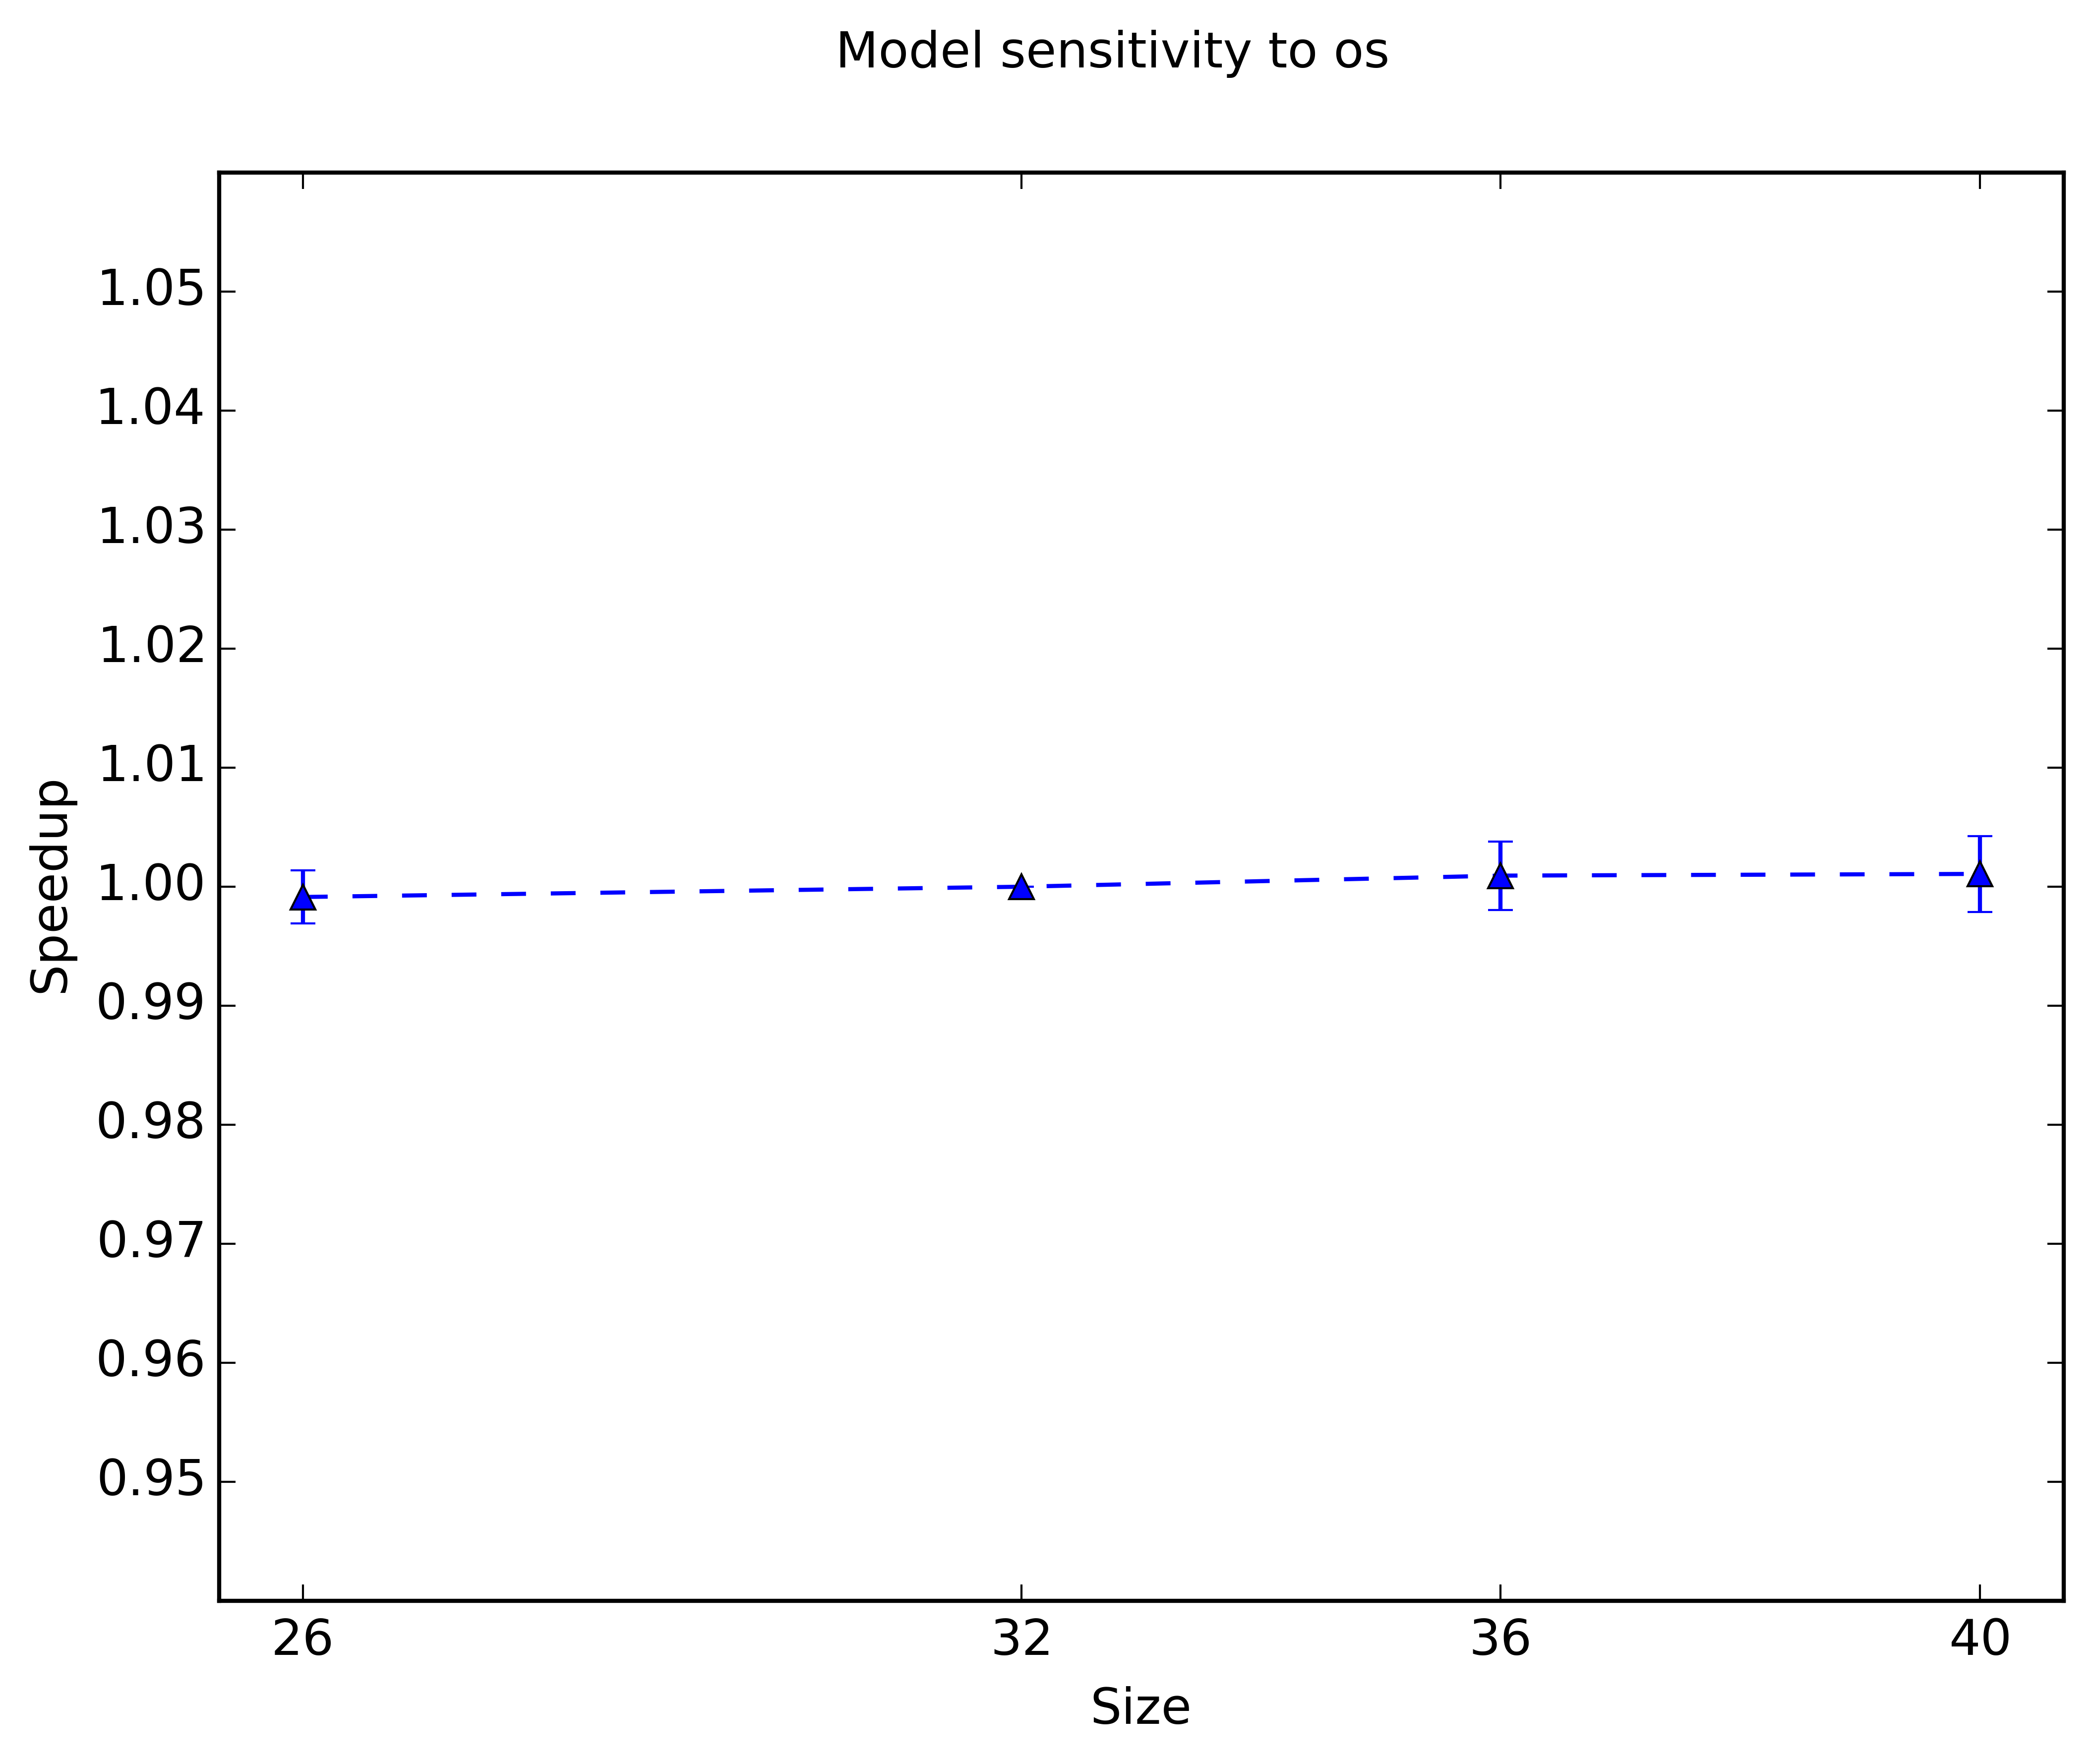
\includegraphics[width=\textwidth]{figures/processor_model/os}
                \caption{Outstanding Stores.}
                \label{fig:results:processor_model:os}
        \end{subfigure}
        \begin{subfigure}[b]{0.5\textwidth}
                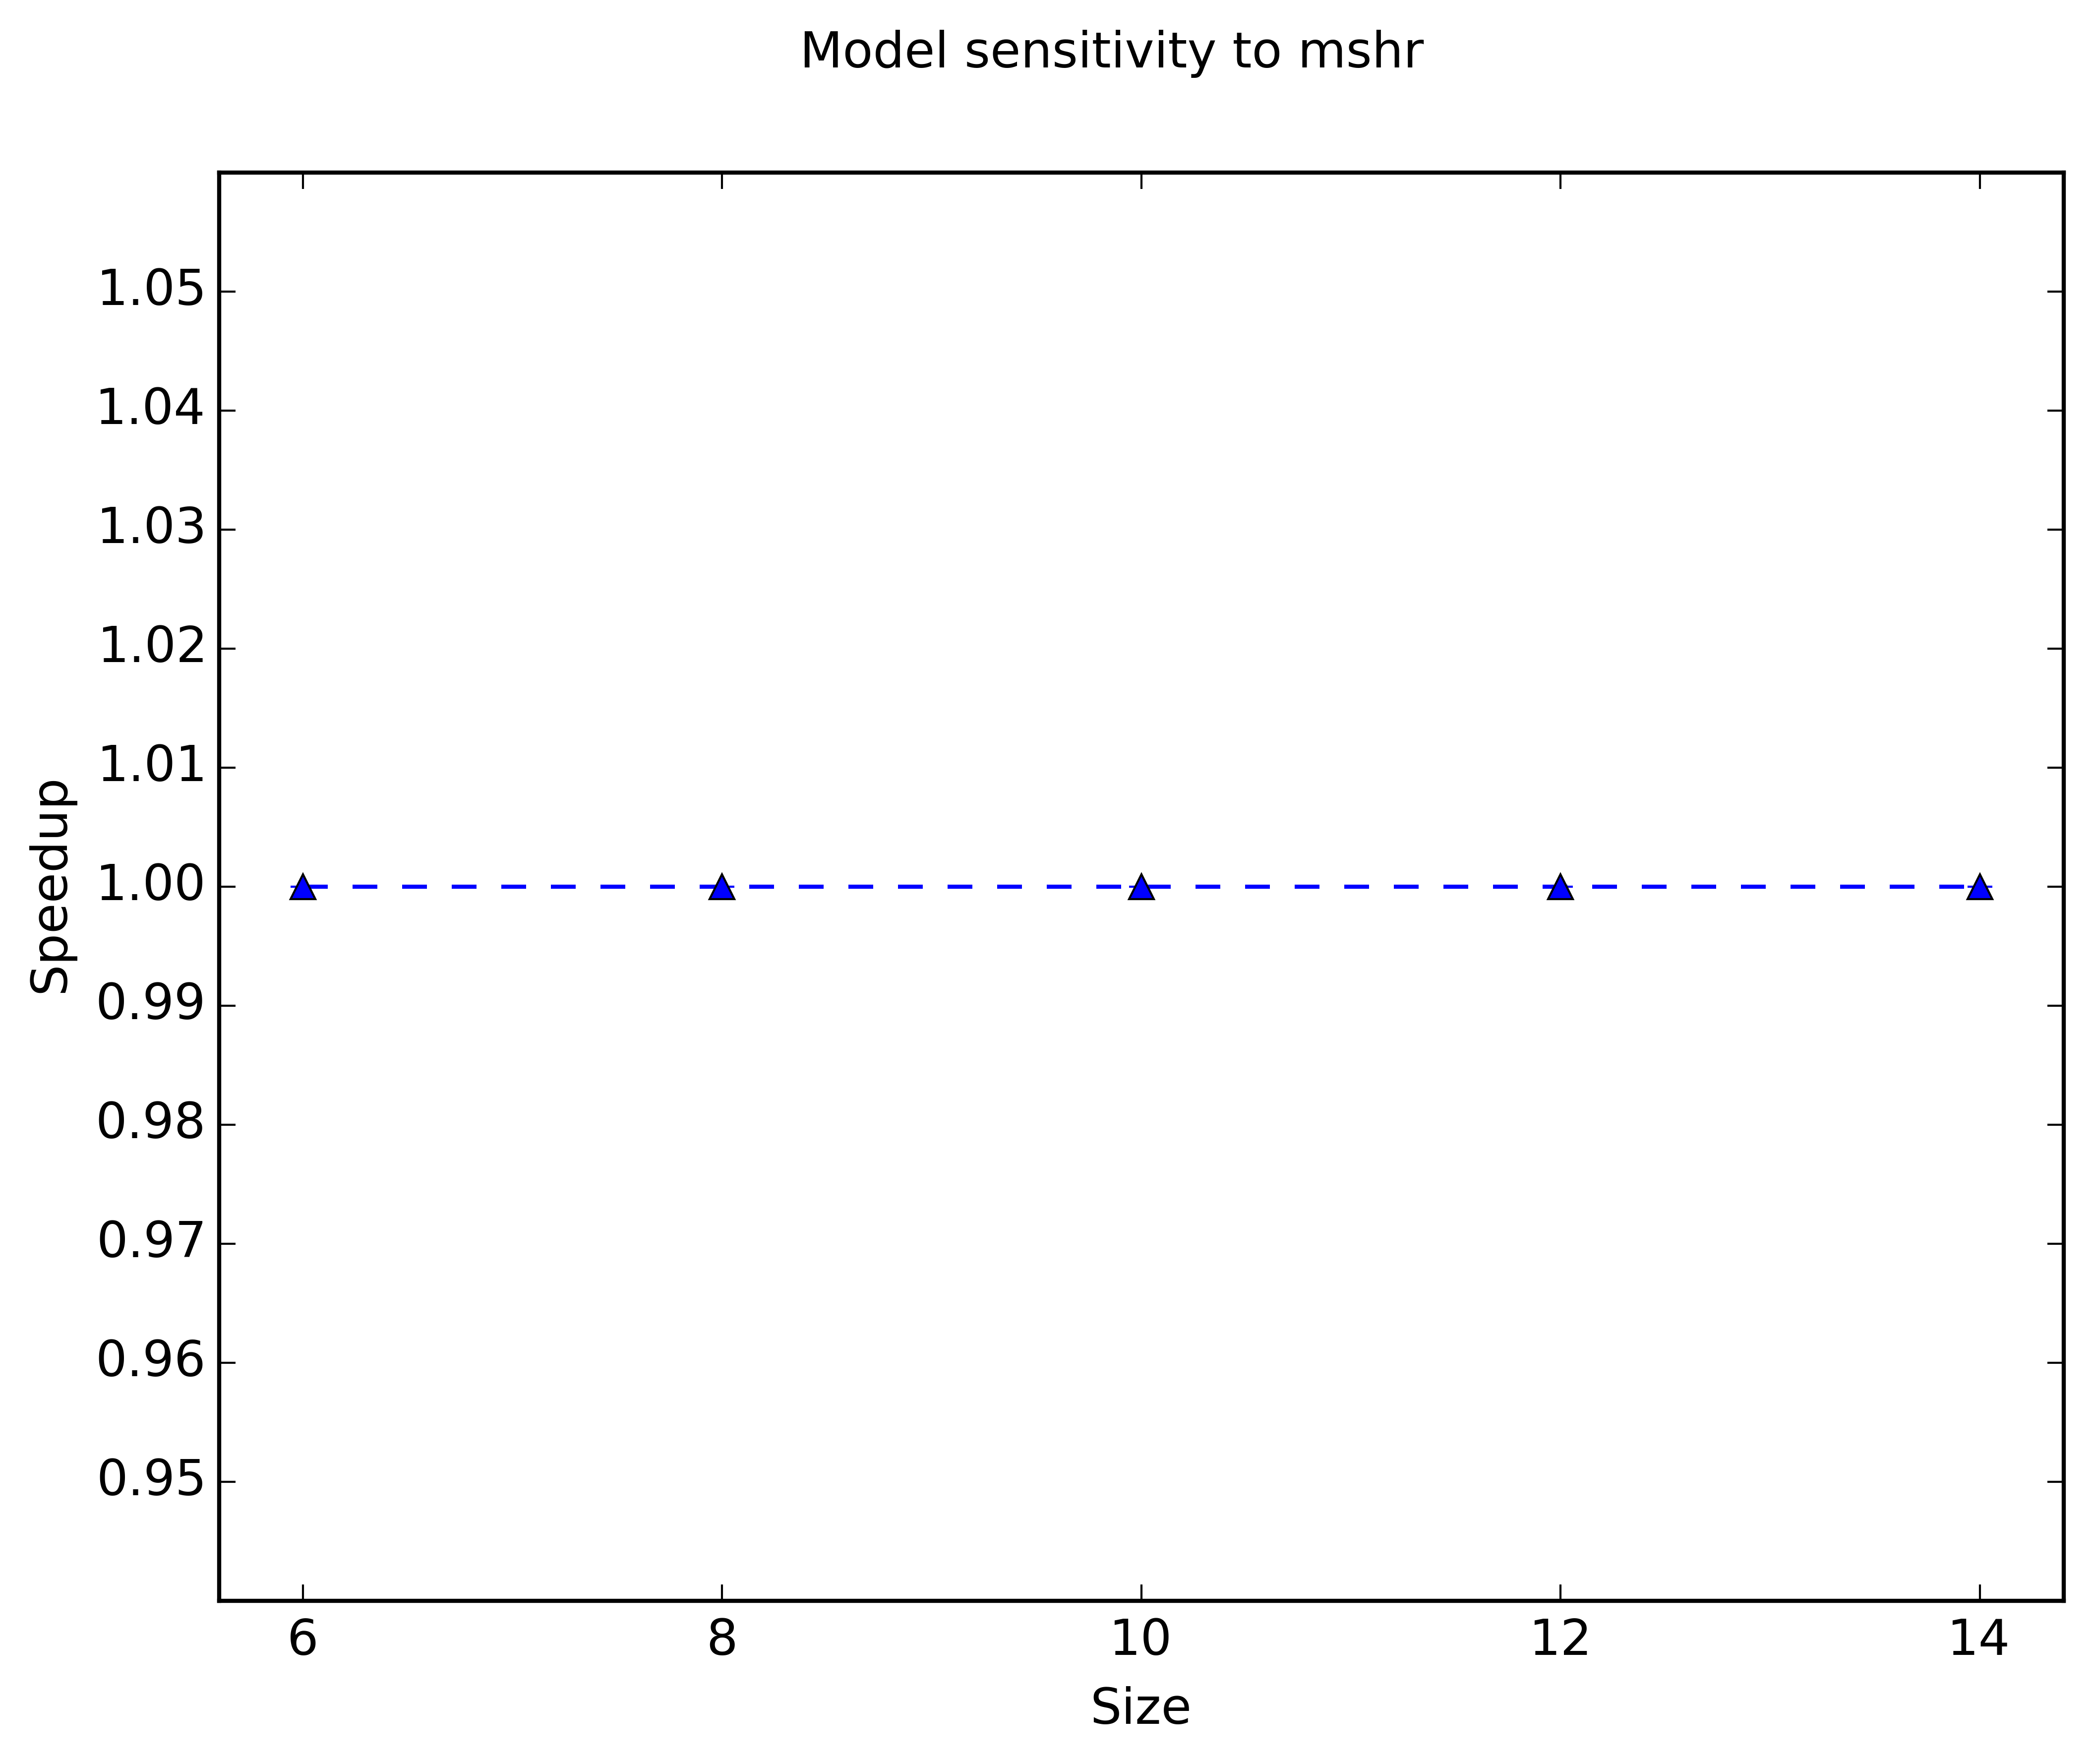
\includegraphics[width=\textwidth]{figures/processor_model/mshr}
                \caption{L1 Miss Status Hold Register.}
                \label{fig:results:processor_model:mshr}
        \end{subfigure}%
        \begin{subfigure}[b]{0.5\textwidth}
                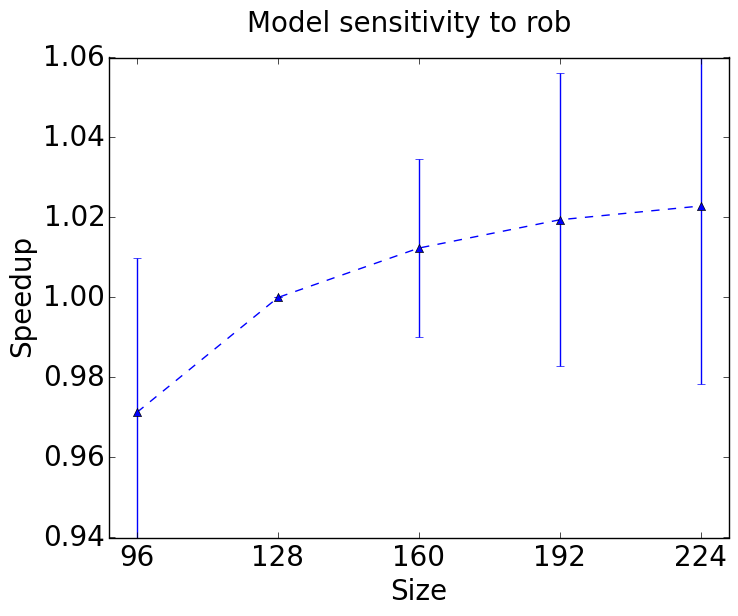
\includegraphics[width=\textwidth]{figures/processor_model/rob}
                \caption{Re-order Buffer.}
                \label{fig:results:processor_model:rob}
        \end{subfigure}
        \begin{subfigure}[b]{0.5\textwidth}
                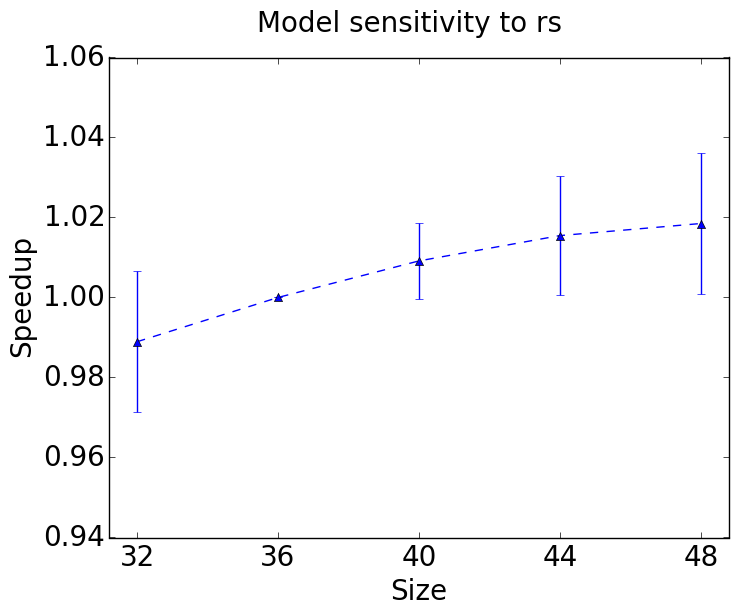
\includegraphics[width=\textwidth]{figures/processor_model/rs}
                \caption{Reservation Station.}
                \label{fig:results:processor_model:rs}
        \end{subfigure}%
        \caption{Core model property sensitivity.}
        \label{fig:results:processor_model}
       ~ % Fill page, prevents latex from placing a single line of text under the figure
\end{figure}

Figure~\ref{fig:results:processor_model} shows the average speedup of all benchmarks when we vary our five selected properties; Outstanding loads (ol), outstanding stores (os), L1 \gls{mshr}, re-order buffer size (rob) and reservation station entries (rs).
Outstanding loads and stores specify the number of outstanding memory requests the core can have active in the rob.
The number of L1 \glspl{mshr} decide how many outstanding cache misses the first level cache can handle before it has to block on a miss.
The size of the rob and rs together decide how many instructions can be live during execution.  
Increasing the number of live instructions can increase the amount of \gls{ilp} the processor can extract from the program while possibly increasing the cost of a branch miss prediction.

For two of the memory related properties; os and ol, we observe no improvement nor decrease in performance for the values we explored.
When we increase the last memory related parameter, \gls{mshr}, we do observe a slight performance change.
With an increasing number of \glspl{mshr}, the cache and hence the core can handle more outstanding memory requests. 
As a result, the core will be able to exploit more \gls{ilp}, and a slight performance improvement is observed. 
Unlike the \glspl{mshr}, we do not expect the value of os and ol to affect performance. 
If the core is to gain performance from supporting more outstanding loads there has to be more than 48 loads among the 128 instructions that fit in the rob. 
Equally there must be more than 32 stores per 128 instructions for an increased os limit to be beneficial.
Also, both os and ol are limited by the number of memory requests the memory system can handle, and the total number of L1 \glspl{mshr} is less than the size of both os and ol.
The observed performance gain when increasing the number of \glspl{mshr} in the first level caches, as seen in Figure~\ref{fig:results:processor_model:mshr}, is less than 1\% with a 50\% storage increase. 
We also observe a standard deviation of more than 3\%. 

When Increasing the size of the rob and the number of rs entries, we observe a slight increase in performance.
Figures~\ref{fig:results:processor_model:rob}~and~\ref{fig:results:processor_model:rs} show an average performance increase of about 2\% with more rob entries, and about a 3\% increase with more rs entries.
We observe that these increases come at the cost of a 75\% and 50\% storage increase respectively.
Also, we observe that the standard deviation in both cases is about the same as the average performance increase.

When reviewed, these results lead us to conclude that the processor model we have presented, based on the Nehalem architecture, is stable and that we have no obvious performance gains from small adjustments.
As a result, we decide to continue using this model for the rest of our experiments without making any adjustments.

Considering that we base our model on an actual architecture and that our simulator strives to simulate the core model of that same architecture, it is not a far-fetched result observing little sensitivity to property changes.
During the design process of the architecture, it is natural to expect that the designers made a conscious choice between speed and area using a similar analysis.
The final properties would then most likely have been selected to provide a stable middle ground, which we see reflected in our simulation results.